%%
%% This is file `template-msc-classic.tex',
%% generated with the docstrip utility.
%%
%% The original source files were:
%%
%% hecthese.dtx  (with options: `gabarit,msc,classique,anglais')
%% 
%% This is a stripped version of the original file.
%% 
%% Copyright 2017-2019 HEC Montreal
%% 
%% This work may be distributed and/or modified under the
%% conditions of the LaTeX Project Public License, either version 1.3c
%% of this license or (at your option) any later version.
%% 
%% The latest version of this license is in
%% http://www.latex-project.org/lppl.txt
%% and version 1.3c or later is part of all distributions of LaTeX
%% version 2008/05/04 or later.
%% 
%% This work has the LPPL maintenance status `maintained'.
%% 
%% The Current Maintainer of this work is Benoit Hamel
%% <benoit.2.hamel@hec.ca>.
%% 
%% This work consists of the files hecthese.dtx and hecthese-fr.ins,
%% hecthese-en.ins, hecthese.pdf, hecthese-en.pdf
%% and the derived files listed in the README file.
%% 
%% TEMPLATE FOR A CLASSIC THESIS
%%
%% This is the master file where you write all your work-related metadata,
%% where you create your homemade commands and environments. It is from this
%% file that you run your compilations.
%%
%% DO NOT WRITE YOUR DISSERTATION OR THESIS IN THIS FILE!
%%
%% Read the hecthese class documentation for more information.
%%
%% DOCUMENT CLASS DECLARATION
%%
%% The document class is declared with its default document type and
%% language. Write in the options list the desired font size (10pt, 11pt,12pt)
%% or let the class load the default font size: 12pt.
\documentclass[mscclassique,frenchb,english]{hecthese}
%%
%% LOADING PACKAGES
%%
%% Add all the packages you need to write your dissertation or thesis.
%% Read the class documentation so learn more about preloaded packages. Make
%% sure to follow these instructions:
%%
%% 1) The hyperref MUST ALWAYS BE LOADED LAST if you want the package to work
%% correctly.
%% 2) The geometry package et INCOMPATIBLE with the memoir class. You can't
%% use it in your work. Read the memoir class' documentation for more
%% information.
%%
%% CHOOSING A FONT
%%
%% Choose the mathptmx package if you want to use a serif-type font, like
%% Times, and the mathpazo package if you want to use a sans serif-type font,
%% like Arial. Choose one package and delete the other, or comment it out.
\usepackage{mathptmx}
%% \usepackage{mathpazo}

\usepackage{hyperref}
%%
%% INDEX PRODUCTION
%%
\makeindex
%%
%% BIBLIOGRAPHY STYLE
%%
%% We use the default apa bibliography style. Using this style isn't mandatory.
%% Read the class' documentation to learn more about the styles compatible with
%% the language of your dissertation or thesis.
%%
\bibliographystyle{apa}
%%
%% All document divisions up to the subsections are included in the table
%% of contents. If you want a more detailled table of contents, change
%% the following two commands so they match the level of detail you want
%% in your TOC.
%%
\setsecnumdepth{subsection} % Numérotation des sous-sections / Subsection numbering
\settocdepth{subsection} % Inclusion des sous-sections dans la TDM / Including subsections in the TOC
%%
%% DOCUMENT METADATA
%%
%% The title of your work. If the title is too long, use the \\ command
%% to output the title in multiple lines.
\HECtitle{Dissertation or thesis title}
%% The subtitle of your work. If there is no subtitle, empty the contents
%% from  the curly braces.
\HECsubtitle{Dissertation or thesis subtitle}
%% The author is you...
\HECauthor{FirstName LastName}
%% Name of the M.Sc. or Ph.D. option
\HECoption{Option Name}
%% Month of the work's final submission
\HECsubMonth{May}
%% Year of the work's final submission
\HECsubYear{2018}
%%
%% PACKAGE OPTIONS
%%
%% If your packages need to have options loaded before the document's
%% beginning, write them hereafter. If you want to override preloaded
%% packages' options, read the class documentation to learn how.
%%
%% Options du package hyperref (inclure les métadonnées pdf dans les options) /
%% hyperref package option (including pdf metadata)
\hypersetup{%
colorlinks=true,
allcolors=black,
pdfauthor=\HECpdfauteur,
pdftitle=\HECpdftitre
}
%% Options de babel / babel options
\frenchbsetup{% 
og=«, fg=» % caractères « et » sont les guillemets
}
%%
%% BEGINNING OF THE DISSERTATION OR THESIS
%%
\begin{document}

%% Pages liminaires / frontmatter
\frontmatter

%% Page de garde / cover page
\mbox{}
\thispagestyle{empty}
\cleardoublepage

%% Page de titre
 \HECtitlepages


%% Résumé français / french abstract
 %% File containing the french abstract, keywords and research methods.
\chapter*{Résumé}
\phantomsection\addcontentsline{toc}{chapter}{Résumé}
\thispagestyle{empty} % Première page non paginée / Unnumbered first page

%% Write your french abstract here (350 to 500 words).

\section*{Mots-clés}

%% Write your french keywords here (15 max, including the research methods).

\section*{Méthodes de recherche}

%% Write your research methods here.

%% DISSERTATIONS AND THESES WRITTEN WITH ARTICLES
%% If you have inserted citations in this section, uncomment the following
%% command and type in the bibliography style and the .bib file name
%% used for your references.
%% \HECreferences{style}{nom-du-fichier-file-name}


%% Résumé anglais / english abstract
 %% File containing the English abstract, keywords and research methods.
\chapter*{Abstract}
\phantomsection\addcontentsline{toc}{chapter}{Abstract}

%% Write your english abstract hereafter (350 to 500 words).

\section*{Keywords}

%% Write your english keywords here (15 max, including the research methods)

\section*{Research methods}

%% Write your research methods here.

%% DISSERTATIONS AND THESES WRITTEN WITH ARTICLES
%% If you have inserted citations in this section, uncomment the following
%% command and type in the bibliography style and the .bib file name
%% used for your references.
%% \HECreferences{style}{nom-du-fichier-file-name}


%% Table des matières (* pour ne pas inclure la TDM dans la TDM) /
%% Table of contents (* for excluding the TOC from the TOC)
\tableofcontents*
\cleardoublepage

%% Liste des tableaux / list of table
\listoftables
\cleardoublepage

%% Liste des figures / list of figures
\listoffigures
\cleardoublepage

%% Liste des abréviations / acronyms list
 %% File containing the acronyms list. You'll find below and example list. The
%% HECabbreviations environment takes as an argument the longest acronym. On
%% compilation, a list with two aligned columns is generated.
\chapter*{\HECtdmAbreviations}
\phantomsection\addcontentsline{toc}{chapter}{\HECtdmAbreviations}

\begin{HECabbreviations}{ABBR}
\item[ABBR] Abréviation
\item[BAA] Baccalauréat en administration des affaires
\item[DESS] Diplôme d'études supérieures spécialisées
\item[HEC] Hautes études commerciales
\item[MBA] Maîtrise en administration des affaires
\item[MSc] Maîtrise
\item[PhD] Doctorat
\end{HECabbreviations}


%% Avant-propos / preface
 %% File containing the preface
\chapter*{\HECtdmAvantPropos}
\phantomsection\addcontentsline{toc}{chapter}{\HECtdmAvantPropos}

%% Write your preface here.

%% DISSERTATIONS AND THESES WRITTEN WITH ARTICLES
%% If you have inserted citations in this section, uncomment the following
%% command and type in the bibliography style and the .bib file name
%% used for your references.
%% \HECreferences{style}{nom-du-fichier-file-name}


%% Remerciements / acknowledgements
 %% File containing the acknowledgements
\chapter*{\HECtdmRemerciements}
\phantomsection\addcontentsline{toc}{chapter}{\HECtdmRemerciements}

%% Write your acknowledgements here.


%% Partie principale de la thèse ou du mémoire / mainmatter
\mainmatter

%% Introduction
\chapter{Introduction}
This is a template for writing a thesis according to the Technion specifications. 
Please, however, check with the graduate school website to see if any specifications have changed. 
This template was written by Boaz Shuval (January 2019). 

\section{Instructions}

This template is provided as is. Please check with the Technion graduate school website to see if the guidelines have changed, as they often do. For
the latest directions from the graduate school, see: 
\url{https://graduate.technion.ac.il/graduation/thesis-editing/}
(This is the website address circa January 2019). 

All files use UTF-8 encoding. Make sure your LaTeX system supports this encoding. 

\subsection{Preparing the Thesis}

\begin{enumerate}
\item The main.tex file is the main file to be compiled. Place it (with the other thesis files) in the same directory as the \verb".cls" and \verb".sty"
    files provided.                                                                                                                                          
    \item  The main class is \verb"technionThesis.cls."
   It has the the following options:  
   \begin{itemize}
       \item  hyperref       ---  Add hyperlinks
       \item  publist        ---  Add a list of publications in the front pages (update list in thesissetup.sty)
       \item  addack         ---  Add an acknowledgments page (only for final version!)
       \item  advisement     ---  Use "advisement" instead of "supervision" in front pages (a pet peeve of mine)
       \item  spacepar       ---  Add a blank line between paragraphs
       \item  firstparindent ---  Indent the first paragraph of a chapter/section
       \item  libertine      ---  Use a different selection of fonts, based on libertine, for the English part of the thesis. (See note 4)
    \end{itemize}
\item In the file \verb"technionThesisSetup.sty" you must input your details in the various commands. It is pretty self explanatory. 
\item The class loads a number of packages that the class author (Boaz Shuval) uses regularly. It also sets up theorem-style environments.
   If you know what you're doing, feel free to change things as you see fit. Otherwise, leave this alone. 
   \begin{enumerate}
       \item Environments are defined using amsthm. The following environments are available:
           \begin{itemize}
               \item Theorem-style: theorem, lemma, corollary, proposition, conjecture
      (Heading in bold, text in italics)
      These all share consecutive numbering, in the format (chapter.number)
  \item Definition-style: definition, example, assumption, condition 
      (Heading in bold, text upright)
      These are numbered (chapter.number) with their own numbering. Assumption and condition have alphanumeric numbering (A,B,C, etc.)
  \item Remark-style: remark, question, discussion
      (Heading in italics, text upright)
      These are numbered (chapter.number) with their own numbering. Discussion is unnumbered. 
  \item Proof environments: proof, IEEEproof. Both have a black square at the proof end. 
    \end{itemize}
\item  Packages loaded (partial listing):
    \begin{itemize}
        \item mathtools (which loads amsmath)
        \item amsthm, amssymb
        \item IEEEtrantools (loads IEEEeqnarray, and also sets the bibliography style)
        \item graphicx 
        \item tikz (including various useful tikz libraries) 
        \item cleveref (for referring to sections, etc, using \verb"\Cref", automagically adding the header)
        \item stackrel
        \item accents  (for adding symbols above symbols)
        \item xspace (for adding a smart space after a macro command)
        \item tabto  (add a tabstop for lining things up)
        \item algorithm2e (ruled, vlined)
        \item url
        \item polyglossia (for Hebrew support)
        \item longtable (for a table that runs over more than one page; useful for the abstract)
        \item booktabs, multirow (for nicer tables)
    \end{itemize}
    \end{enumerate}
\item Place all of your own commands in the file \verb"Example/technionThesisMacros.sty". That is, various \verb"\newcommand" and \verb"\DeclareMathOperator" are defined here. I've defined a few
   useful ones for you to get started. 
\item There are now \verb".tex" files for you to edit: 
    \begin{itemize}
        \item \verb"abstract.tex"         for your abstract in English (200-500 words)
        \item \verb"habstract.tex"        for your abstract in Hebrew (500-2000 words)
        \item \verb"acknowledgments.tex"  for your acknowledgments in English
        \item \verb"hacknowledgments.tex" for your acknowledgments in Hebrew
        \item \verb"introduction.tex"     for your introduction chapter
        \item \verb"chapfirst.tex"        for your first chapter 
        \item \verb"chapsecond.tex"       for your second chapter (add additional chapters as you see fit)
        \item \verb"discussion.tex"       for your discussion/conclusions chapter
        \item \verb"appendix.tex"         for your appendix (appendices must appear in their own chapters, and not as part of the main text). 
   \end{itemize}
   \end{enumerate}

   \subsection{Compilation}
Compile using xelatex. If you are using latexmk, you may include in the compilation directory a file called \verb".latexmkrc"
with the following line: 

\verb"$pdflatex = 'xelatex --shell-escape %O %S';"

This tells latexmk to use xelatex for compilation, so you need not worry
about this.
You may also compile this on overleaf (again, use xelatex). 

The Hebrew portion of the thesis is based on the polyglossia package. It uses the David CLM font for Hebrew. Thus, you must install the culmus fonts
for this to work on your installation. 

\subsection{ Be a pal}
Please share this template with your friends and colleagues. 
If you enjoyed using it, consider sending me a note to let me know. 
If you find a bug, or have asuggestion for improvement, I'd love to know about it.

\section{Files in this Template}

\begin{itemize}
    \item  \verb"technionThesis.cls"     ---  The class file
    \item  \verb"technionThesisSetup.sty"        ---  Setup data fields
    \item  \verb"README.md"                
    \item  Inside the Example directory:
        \begin{itemize}
    \item  \verb"abbrev.tex"               
    \item  \verb"abstract.tex"             
    \item  \verb"acknowledgments.tex"
    \item  \verb"appendix.tex"
    \item  \verb"chapfirst.tex"
    \item  \verb"chapsecond.tex"
    \item  \verb"discussion.tex"
    \item  \verb"habstract.tex"          ---  Hebrew abstract
    \item  \verb"hacknowledgments.tex"   ---  Hebrew acknowledgments
    \item  \verb"introduction.tex"
    \item  \verb"main.tex"               ---  Main thesis file
    \item  \verb"mybib.bib"
    \item  \verb"technionThesisMacros.sty"           ---  Define your macros here
\end{itemize}
\end{itemize}

\section{License}
This template is licensed under Creative Commons CC BY 4.0. 

\section{Notes}
\begin{enumerate}
    \item This template was tested on a mac running macOS 10.13, with TEXLIVE2017. It was also tested on overleaf in January 2019, which also runs TEXLIVE2017. 
    \item There is a bug when using TEXLIVE2018, which manifests itself in the figure/table numbering. If you encounter this bug, use the memoir package from
          TEXLIVE2017, instead. 
    \item The template uses the Memoir package internally. The chapter heading design is a modified version of a design by Vincent Zoonekynd 
        (it is modified from the BlueBox style in \url{https://ctan.org/pkg/memoirchapterstyles}).  
       \item If using the libertine option, make sure to use the latest version of newtxmath, available from \url{https://ctan.org/pkg/newtx}
   (download the file \verb"newtxmath.sty" to the home directory)
   \end{enumerate}


   \section{ Version History}
31 January 2019:    Version 1.0




\section{A Section} 
The remainder of this file is a boilerplate example
Equations are also fine: 
\[ 
    f(x) = x+2,
\] 
as are numbered equations:
\begin{equation}\label{eq:numbered int}
    g(y) = y.
\end{equation}
Of course, one may refer to a numbered equation such as~\eqref{eq:numbered int}. 

\section{Second section}
In this section we have a figure. 

\begin{figure}[t]
    \begin{center}
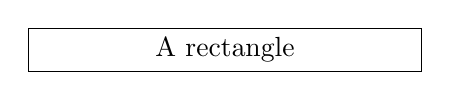
\begin{tikzpicture}
    \node[draw, minimum width = 5cm] {A rectangle};
\end{tikzpicture}
\end{center}
\caption[Short caption]{A very long caption for this figure. It is deliberately very long to illustrate the usefulness of the short caption for the table of figures. }
\label{fig:rectangle}
\end{figure}
\lipsum[10-13]

















%% Revue de la littérature / literature review
 %% File containing the literature review
\chapter*{\HECtdmRevueLitterature}
\phantomsection\addcontentsline{toc}{chapter}{\HECtdmRevueLitterature}
\thispagestyle{empty} % Première page non paginée / First page unnumbered

%% Write your literature review here.

%% DISSERTATIONS AND THESES WRITTEN WITH ARTICLES
%% If you have inserted citations in this section, uncomment the following
%% command and type in the bibliography style and the .bib file name
%% used for your references.
%% \HECreferences{style}{nom-du-fichier}


%% Chapitres de développement / chapters
%% File containing one of the main content's chapters. The class
%% generates three chapter files by default. If you need more,
%% save a file with another name and include it in your template file
%% with the \include command.
\chapter{Titre du chapitre / Chapter title}
\thispagestyle{empty} % Première page non paginée / First page is unnumbered

%% Write your chapter here.

\include{chapter-2}
\include{chapter-3}

%% Conclusion
%% Fichier contenant la conclusion
\chapter*{\HECtitreConclusion}
\phantomsection\addcontentsline{toc}{chapter}{\HECtitreConclusion}
\thispagestyle{empty} % Première page non paginée / First page is unnumbered

%% Rédigez votre conclusion ici.

%% THÈSES ET MÉMOIRES PAR ARTICLES SEULEMENT
%% Si vous avez inséré des citations dans cette section, retirez les signes
%% de commentaires (%%) devant la commande ci-dessous et inscrivez le style
%% bibliographique et le nom du fichier .bib utilisés pour vos références.
%% \HECreferences{style}{nom-du-fichier-file-name}


%% Index analytique / analytical index
\printindex

%% BIBLIOGRAPHIE / BIBLIOGRAPHY
%% Write the name of your .bib file between the curly braces.
\bibliography{}

\backmatter

%% Retour à la pagination romaine / Back to roman page numbering
\pagenumbering{roman}

%% Annexes / appendices
\appendix
 %% File containing an appendix. The class only generates one appendix by default.
%% If you need more, save the file with another name and include in your
%% template file with the \include command.
%%
%% For the bibliography and appendices to be paged correctly, meaning in arabic
%% numbers for the bibliography and roman numbers for the appendices, the latter
%% have to placed after the \backmatter command. But by doing so, the appendices'
%% numbering will be disabled. You'll have to number your appendices manually
%% inside the \chapter command.
\chapter{Appendix A -- Appendix Title}

%% Write your appendix here.

%% DISSERTATIONS AND THESES WRITTEN WITH ARTICLES
%% If you have inserted citations in this section, uncomment the following
%% command and type in the bibliography style and the .bib file name
%% used for your references.
%% \HECreferences{style}{nom-du-fichier-file-name}


%% Page de garde de fin / back cover page
\mbox{}
\thispagestyle{empty}

\end{document}
\endinput
%%
%% End of file `template-msc-classic.tex'.
